\chapter{Introduzione al nucleo didattico}
Il nucleo didattico è un \textbf{kernel a 64 bit} perfettamente funzionante, utilizzato per finalità didattiche nel corso di Calcolatori Elettronici di Ingegneria Informatica presso l'Università di Pisa e sviluppato a partire dai concetti presentati in \citetitle{frosini:calcolatori3} di \citeauthor{frosini:calcolatori3}\cite{frosini:calcolatori3}.

Il sistema è organizzato in tre moduli distinti \cite{lettieri:nucleo}:
\begin{itemize}
	\item \textbf{SISTEMA}, eseguito con il processore a livello sistema, che contiene la realizzazione dei processi, inclusa la gestione della memoria;
	\item \textbf{IO}, eseguito con il processore a livello sistema, che contiene le routine di ingresso/uscita che permettono di utilizzare le periferiche collegate al sistema;
	\item \textbf{UTENTE}, eseguito con il processore a livello utente, che contiene il programma che il nucleo dovrà eseguire.
\end{itemize}
I moduli sistema e io forniscono un supporto al modulo utente, sotto forma di \emph{primitive} che questo può invocare.

Il sistema sviluppato, per quanto funzionante, non è autosufficiente e per sviluppare i moduli necessita di un altro sistema di appoggio, nel nostro caso Linux, i cui strumenti devono essere opportunamente configurati in modo che produca eseguibili per il nostro sistema. Il nucleo così sviluppato può essere eseguito sia su una macchina reale (sconsigliato), sia su un emulatore. Nel nostro caso, useremo una versione di QEMU opportunamente modificata~\cite{lettieri:istruzioni-nucleo}.

Il modulo sistema deve essere caricato da un \emph{bootstrap loader} mentre il modulo io e utente devono essere caricati da una \emph{partizione di swap}, nel nostro caso emulata da un file binario

\section{Gestione dei processi}
All'interno del nucleo didattico, i processi vengono rappresentati attraverso due strutture dati:
\begin{itemize}
	\item Il descrittore di processo (\emph{des\_proc}), contenente il TSS del processo e i valori dei registri salvati all'ultimo cambio di contesto. Viene indirizzato dalla entrata della GDT relativa al processo.
	\item Il \emph{proc\_elem}, contenente l'id e la priorità del processo e usato nelle code di processi.
\end{itemize}

Il sistema prevede una politica di schedulazione a priorità fissa, in cui passa in esecuzione il processo pronto con priorità \emph{maggiore}. A parità di priorità, viene adottata una politica FIFO (\emph{First Input, First Output}).

\section{Gestione della memoria virtuale}
Il nostro sistema implementa la paginazione su domanda~\cite{lettieri:paginazione-su-domanda}, con zone di memoria condivise tra tutti i processi e zone private ai processi~\cite{lettieri:paginazione-nel-nucleo}.

\begin{figure}
	\centering
	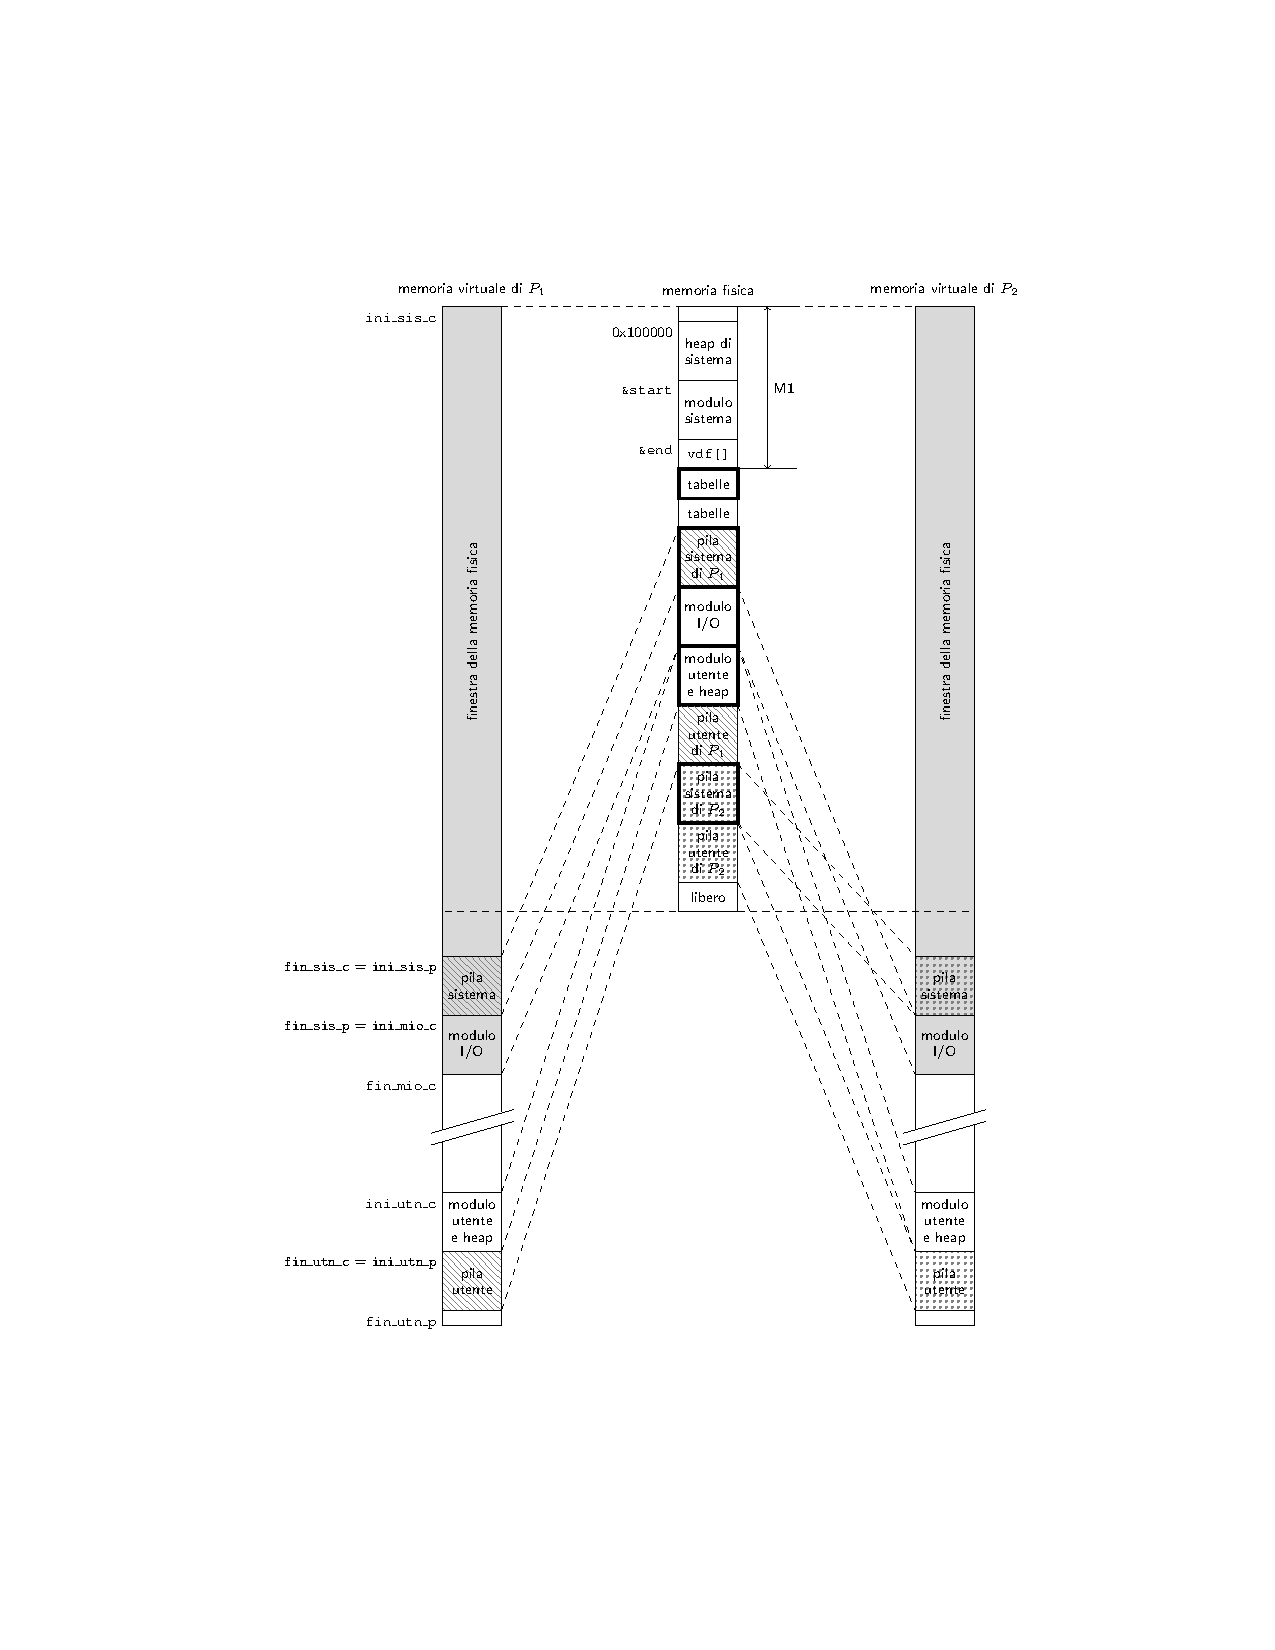
\includegraphics[width=\textwidth]{"img/memoria-virtuale-nucleo.pdf"}
	\caption{Esempio di memoria virtuale con due processi (non in scala)~\cite{lettieri:paginazione-nel-nucleo}}
	\label{fig:memoria-virtuale-nucleo}
\end{figure}

La memoria virtuale di ogni processo è diviso nelle seguenti sezioni (vedi anche \ref{fig:memoria-virtuale-nucleo}: 
\begin{itemize}
	\item Il sottospazio canonico superiore, con indirizzi da 0X0000000000000000 a 0X00007FFFFFFFFFFF, accessibile solo da livello sistema. A sua volta suddiviso in:
	\begin{itemize}
		\item \textbf{sistema/condivisa}: contiene la finestra di memoria fisica
		\item \textbf{sistema/privata}: contiene la pila sistema del processo
		\item \textbf{IO/condivisa}: contiene il modulo I/O
	\end{itemize}
	\item Il sottospazio canonico inferiore, con indirizzi da 0XFFFF800000000000 a 0XFFFFFFFFFFFFFFFF, accessibile solo da livello sistema. A sua volta suddiviso in:
	\begin{itemize}
		\item \textbf{utente/condivisa}: contiene il modulo utente, ovvero le sezioni \texttt{.text} e \texttt{.data} del programma utente
		\item \textbf{utente/privata}: contiene la pila utente del processo
	\end{itemize}
\end{itemize}
Si noti come alcune parti della memoria fisica siano accessibili esclusivamente tramite la finestra: il primo MiB riservato per ragioni storiche, lo heap di sistema, il modulo sistema, i descrittori di frame e i descrittori di pagine virtuali.

Usando la paginazione su domanda, la memoria fisica funziona da cache dello swap. Normalmente le sole sezioni \emph{residenti}, ovvero non selezionabili come vittime per uno swap, sarebbero la \emph{sistema/condivisa} e la \emph{sistema/privata}, in quanto contenenti la finestra di memoria e la pila usata dal modulo sistema. Per semplicità di implementazione, nel nostro sistema sono state rese residenti tutte le sezioni condivise~\cite{lettieri:paginazione-nel-nucleo}.
